\documentclass[12pt,a4paper]{report}
\usepackage{fullpage}
\usepackage[margin=2cm]{geometry}
\usepackage{mathtools,amsmath}
\usepackage{graphicx}
\usepackage[]{algorithm2e}
\usepackage{tikz}
\usepackage{multicol}
\usepackage{subfig}
\begin{document}
\title{Weekly report}
\author{LE Van Linh and BEURTON-AIMAR Marie}
\date{November 2016}
\maketitle
\begin{abstract}
	This document contains the summary about the morphometry and deep learning studied. Besides, it also contains the algorithms to apply for image processing such as segmentation or detection the dominant points.
\end{abstract}
\part{Morphometry}
Morphometry (or morphometrics) is a norm refers to the analysis of form, specifics size and shape of the object in digital image. Morphometry analyses are commonly performed on organisms, and are useful in analyzing the structure of the organisms. Morphometry can be used to extract the general information of creatures, or reconstruct the shape of the organism based on the analysed information that we had. Besides, morphometry can also detect the changes on creatures. Based on these information, we can statically the hypotheses about the factors that affect to the changes of shape.\\[0.2cm]
We have three distinct approaches are usually use: traditional morphometry, landmark-based morphometry and outline-based morphometry.
\begin{enumerate}
	\item Traditional morphometry:  measure the size of the object such as the length, width, angle, ratio and areas on object. The traditional morphomentry is using many measurement of size that most will be highly correlated; as a result, there are few independent variables despite the many measurements.
	\item Landmark-based morphometry: finding enough landmark to provide  a comprehensive description of shape. From the set of beginning landmarks, we can estimate the the missing landmarks.
	\item Outline-based morphometry: a mathematical functions is fitted to points sampled along the outline.
\end{enumerate}
In this part, we will describe the method to analysis the morphometry based on the landmarks. The method is through the several technique in image processing. At the end of this part, a software had built to verify the linkage of the steps.
	\chapter{Segmentation}
\section{Canny algorithm}
In 1986, \textbf{John F.Canny} had proposed a method to determine the edge in image. This is a technique to detect the useful structure of the object in digital image. Until now, the Canny algorithm\cite{canny1986computational} is used widely for the segmentation in computer vision. The process of Canny algorithm can be described in 4 steps as follows:
\begin{enumerate}
	\item Smoothing the image to reduce the noises by using Gaussian filter
	\item Finding the intensity and direction gradient of each pixel in image
	\item Eliminating the weak edge by using the edge thinning technique.
	\item Applying double threshold to determine the potential edges
\end{enumerate}
	\subsection{Gaussian filter}
	To smooth the image, a Gaussian filter is applied to convolve with the image. This step will help to reduce the effects of the noises on the edge detector. Normally, the equation of a Gaussian kernel with size $(2k+1)$ x $(2k + 1)$  is computed as:
	\begin{equation}
	H_{ij}=\frac{1}{2\pi\sigma^2}exp(-\frac{(i-(k+1))^2 + (j-(k+1))^2}{2\sigma^2});1\leq i,j \leq (2k+1)
	\end{equation}
	where $k$ is the size of kernel, and it should be a odd number.\\
	For example, a 3x3 Gaussian filter with $\sigma = 1 $ as followed:
	\begin{equation}
		G = 
		\begin{bmatrix}
		1 & 2 & 1\\
		2 & 4 & 2\\
		1 & 2 & 1		
		\end{bmatrix}
	\end{equation}	
	
	The selection of the size of the Gaussian kernel is important, it will affect the performance of the detector. If the size of the kernel is large, the detector can be sensitive to noise; otherwise, if the kernel's size is small, the detector can be destroy many strong edge. In the practice, this step is combined into Sobel convolution with a 3x3 kernel, which used to finding the intensity and direction gradients at each pixels of image.
	\subsection{Sobel convolution}
	The points belong to the edge in an image can stay in any direction, so the Canny algorithm uses four filters to detect the edges (vertical, horizontal and two diagonal edges) in the image. And the Sobel operator is used to detect the edges. This operator returns a value for the first derivative in horizontal direction $(G_x)$ and the vertical direction $(G_y)$. From these values, the gradient and direction of edge at each pixel are determined:
	\begin{equation}
		G = \sqrt{{G_x}^2 + {G_y}^2}
	\end{equation}
	\begin{equation}
		\phi = atan2(G_y,G_x)
	\end{equation}
	In this case, the kernel of Sobel convolution is 3x3, and it is also combined the Gaussian filter to smooth the image. The kernels are used to convolute the horizontal direction and vertical direction as follows:
	\begin{equation}
		G_x = 
		\begin{bmatrix}
		-1 & 0 & 1\\
		-2 & 0 & 2\\
		-1 & 0 & 1		
		\end{bmatrix}, 
		G_y = 
		\begin{bmatrix}
		-1 & -2 & -1\\
		0 & 0 & 0\\
		1 & 2 & 1		
		\end{bmatrix}
	\end{equation}
	
	The edge direction angle is rounded to one of four angles which were presented for four directions: vertical, horizontal, and two diagonals $0^o, 45^o, 90^o \text{ and } 135^o$.
	\subsection{Non-maximum suppression}
	Non-maximum suppression is applied to thin the edge in an image. Thus, this operation is used to suppress all the gradient values to 0 except the local maximal. At every pixel, it suppress the gradient value of the center pixels if its magnitude is smaller than the magnitude of one out of two neighbors in the gradient direction. In details:
	\begin{itemize}
	\item If the gradient direction angle is \textbf{0} degree, the point will be considered to be on the edge if the gradient magnitude is greater than the magnitude at pixels in the \textbf{east} and \textbf{west} directions.
	\item If the gradient direction angle is \textbf{45} degree, the point will be considered to be on the edge if the gradient magnitude is greater than the magnitude at pixels in the \textbf{north east} and \textbf{south west} directions.
	\item If the gradient direction angle is \textbf{90} degree, the point will be considered to be on the edge if the gradient magnitude is greater than the magnitude at pixels in the \textbf{north} and \textbf{south} directions.
	\item If the gradient direction angle is \textbf{135(-45)} degree, the point will be considered to be on the edge if the gradient magnitude is greater than the magnitude at pixels in the \textbf{north east} and \textbf{south west} directions.
	\end{itemize}
	\subsection{Double threshold}
	After applying the non-maximum suppression, the edges pixels are presented. However, there are still some edge pixels effected by noise. Double threshold will filter out the edge pixels with the weak gradient value and preserve the edge with the hight gradient value.
	\begin{itemize}
		\item A pixel called strong pixel (hence, it belong to the edge), if the edge pixel's gradient value is higher than the high threshold value.
		\item A pixel will be suppressed, if the edge pixel's gradient value is smaller than the low threshold value.
		\item A pixel called weak pixel (can be belong to the edge or not), if the edge pixel's gradient value is larger than low threshold value and smaller than high threshold value. A weak pixel can be belong to the edge if it connected with a strong pixel in 8-connected; else, it will be suppressed.
	\end{itemize}
	Thus, the accuracy of algorithm is depended on two parameters: the kernel of Gaussian filter and thresholds value. As said before, if we choose incorrect the kernel size of Gaussian filter, we can not reduce the noise or we can remove the real edge. Besides, the values of double threshold is also important to filter out the edge pixels. In practice, 1:3 is the good ratio between lower threshold  and upper threshold in Canny.
	\subsection{Summary}
	With applying double thresholding in the last stage, Canny had provied a strict condition to consider the weak edge as well as remove the pixels which were not belong to the edge. So far, Canny algorithm is good method to determined the edge in image, it is used by many application in image processing.
\section{Suzuki algorithm}
The Canny algorithm had detected the edge in the image. We can apply many difference methods to track the edge. \textbf{S. Suzuki} and \textbf{K. Abe}\cite{suzuki1985topological} had proprosed a method to get the border of object in image. This method is based on the topological structure analysis on binary image.\\[0.2cm]
Following this method, it detects two kinds of border in image. The first is outer border, which is defined by a set of border points between an arbitrary 1-component and the 0-component which surrounds it directly; another type is hole border which refers to the set of border points between a hole and the 1-componet which surrounds the hole directly. In this case, the 1-component (or 0-component) is connected component of 1-pixels (or 0-pixels).\\[0.2cm]
In our case, our purpose is getting the edges which were detectecd by Canny\cite{canny1986computational}. An edge is consider as an outer border or a hole border does not important. So, the Suzuki algorithm could make some changes to fit with our aim. The processes of algorithm is desribed as follows:\\[0.2cm]
Let an input binary image is \textbf{$F=\{f_{ij}\}$}. Set initially $NBD = 1$ (denoted the sequence number of border.)
\begin{enumerate}
	\item Select one of the following:
		\begin{enumerate}
			\item If \textbf{$f_{ij} = 1$} and \textbf{$f_{i,j-1} = 0$}, increment NBD, $(i_2,j_2) \gets (i,j-1)$ (pixel $(i,j)$ is the starting point of an outer border).
			\item If \textbf{$f_{ij} \geq 1$} and \textbf{$f_{i,j+1} = 0$}, increment NBD, $(i_2,j_2) \gets (i,j+1)$ (pixel $(i,j)$ is the starting point of an hole border).
			\item Otherwise, go to step (3)
		\end{enumerate}
	\item From the starting point \textbf{(i,j)}, the process to trace the edge is done by substeps following:
		\begin{itemize}
			\item[2.1] Starting from point $(i_2,j_2)$, look around clockwise the pixels in the neighborhood (8-connected) of $(i,j)$ and find the first non-zero pixel $(i_1,j_1)$. If no non-zero pixel is found, assign -NBD to $f_{ij}$ and go to step (3)
			\item[2.2] $(i_2,j_2) \gets (i_1,j_1)$ and $(i_3,j_3) \gets (i,j)$
			\item[2.3] Starting from the \textbf{next element of the pixel $(i_2,j_2)$} in the counterclock-wise order, check the pixels neighborhood of current pixel $(i_3,j_3)$ to find the first non-zero pixel $(i_4,j_4)$.
			\item[2.4] Chang the value $f_{i_3,j_3}$ of the pixel $(i_3,j_3)$ as follows:
				\begin{enumerate}
					\item If the pixels $(i_3,j_3+1)$ is a 0-pixel examined in the substep (2.3) then $f_{i_3,j_3} \gets -NBD$. Else, $f_{i_3,j_3} \gets NBD$ unless $(i_3,j_3)$ is on an already border.
					\item If the pixels $(i_3,j_3+1)$ is not a 0-pixel examined in the substep (2.3) and $f_{i_3,j_3} = 1$ then $f_{i_3,j_3} \gets NBD$
					\item Otherwise, do not change $f_{i_3,j_3}$.
				\end{enumerate}
			\item[2.5] If $(i_4,j_4) = (i,j)$ and $(i_3,j_3) = (i_1,j_1)$ (coming back to the starting point), then go to step (3); otherwise, $(i_2,j_2) \gets (i_3,j3), (i_3,j_3) \gets (i_4,j_4)$ and go back to step (2.3)
		\end{itemize}
	\item Resume the scan from the pixel $(i,j+1)$. The algorithm is stop when the scan reaches the lower right corner of the image.
\end{enumerate}

	\chapter{Dominant points}
In shape analysis, extracting features from the curves is an important step because in another way, we can re-construct the shape from the features. The term dominant points, also called as siginficant points, points of interest, corner points or landmarks is assigned to the points which have the high effect on boundary of object; their dectection is a very important aspect in contours methods because these concentrate the information of a curve on the shape.\\[0.2cm]
Dominant points can be used to produce a presentation of a shape contour for futher processing. The representation ...
In the content of this chapter, we will discuss about the methods to determine the dominant in digital image.\\[0.2cm]
There are many approaches developed for detecting dominant points and the methods can be classified into three groups follows:
\begin{itemize}
	\item Dectermine the dominant points using some significat measure other than curvature
	\item Evaluate the curvature by transforming the contour to the Gaussian scale space.
	\item Search for dominant points by estimating directly the curvature in the original image space.
\end{itemize}
\section{Hough Transform}
One of the challenges in image processing is detecting the characteristic of the object for recognition. Shape recognition is done by searching or detecting a class of simple geometric object such as line, curves in the image and comparing with the model. The matching score of the shapes is calculating by a measurement distance (such as Bhattacharyya). Instead of comparing between the geometric classes from the shapes, we can detect the presence of a shape in anther shape by searching each feature of the shapes. To sovle this problem, Hough Transform (HT)\cite{mukhopadhyay2015survey} is varied. At the beginning, HT\cite{vc1962method} is used to detect the line. It converts the space of parameters from x and y (coordinate of points in line) to space of slope and y-intercept of the line by voting process. For each object statisfying with equation of a line, it votes for the bin have correspondence slope and y-intercept. The set of bins is called the accumulator.
\subsection{Generalizing Hough Transform}
Until now, HT is still a good method for line detection or object recognition. But one of the weakness of HT is cannot determine the end points of the line segments. For this reason, the Generalized Hough Transform (GHT), introduced by Ballard\cite{ballard1981generalizing} is a generalization of HT to detect non-parametric curves. The process includes two phases: learning and recognition. In learning phase, a R-table is construct for model object. R-table is constructed based on the geometric information of each points in curves of object model with a reference point. The reference point can be arbitrary point in the model. Each row in R-table includes the gradient direction of each point which was chosen as index of table; and the polar coordinate values of each point. This mean that a gradient direction can be having many polar coordinate values. During recognition phase, an accumulator is created, called Hough Space. For each point in the scene object, finding the correspondce gradient direction in the R-table and voting at all the coordinate values. The peak in accumnulator is position of reference point of the model object in the scene object. And the peak value is equal to the number of boundary points of the object  when the model and the scene match perfectly.\\[0.2cm]
During recognition phase, the translation and rotation between model object and scene object is determine by principal component axis. Based on the curve points of the object, the centroid of each object is calculated. Then, the principal axis of each object is indicated. The translation between two objects is difference of two centroid points. The angle to rotate is the angle difference of two axes.\\[0.2cm]
When model and scene are matching, the dominant points (landmarks) of scene object is estimated from landmarks of model object by applying the translation, rotation from the centroid points. The last result is verifying by apply template matching (which will discuss as section \ref{template}).
\subsubsection{Result}
Using GHT to extract the landmarks on beetle is experiment on 287 images of right mandible of beetle. To compare the matching between the location of manual landmarks and estimated landmarks, the centroid size is compute for each set of landmarks.\\[0.2cm]
\begin{figure}[h!]
\centering
\subfloat[Model 28]{\label{figpca1}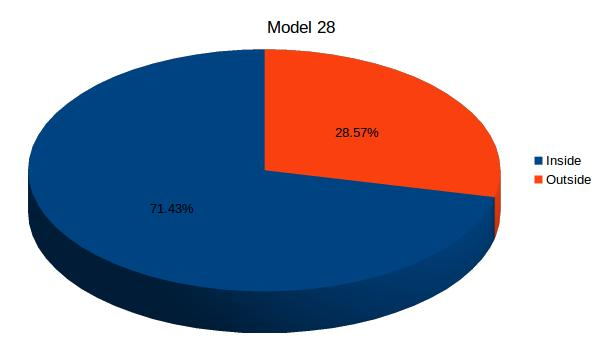
\includegraphics[width=0.5\textwidth]{./images/cmodel28}}~~
\subfloat[Model 71]{\label{figpca2}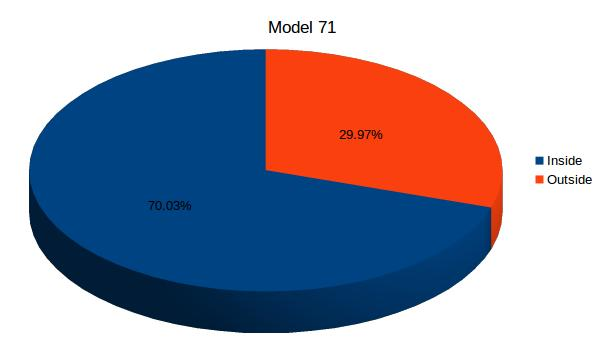
\includegraphics[width=0.5\textwidth]{./images/cmodel71}}
\caption{The accuracy of centroid size on mandible}
\label{figpca}
\end{figure}
Figure \ref{figcentroidSize} display the accuracy of the centroid size of estimated landmarks when we compare with the centroid size of manual landmarks. We use 2 images (Md28.JPG and Md71.JPG) as model. The number of landmarks be detected on scene object is 100\%. For model 28, 71.43\% the centroid of estimated landmarks is placed inside the standard deviation (SD) of manual landmarks, 28.57\% is outside the SD. The ratio for model 71 are 70.03\% and 29.97\%.
\subsection{Probabilistic Hough Transform}
To speed up Hough Transform, instead of processing on all data set, we can consider a subset of data points. The popular method is  \textbf{Probabilistic Hough Transform}. Probabilistic Hough Transform (PHT) is used to detect the presence of a model image in a scene image based on the group of features. The hypothesised location of the model image in the scene image is indicated based on the conditional probability that any pair scene lines agreement about a position in model image. Applying PHT can be separated into two steps: firstly, recording the information of model image and try to find the presence of the model image in scene image (called training process); secondly, predicting the pose of model image in the scene image (called estimating process).\\[0.2cm]
During training process, choose an arbitrary point in the model image, called reference point. For each pair of lines in model image, the perpendicular distance and angle from each line to reference point is recording (angle is calculated as angle between line and a horizontal line begin from reference point). The presence of model image in scene image is detected by PHT with \textit{``vote"} procedure. Finally, we choose the similar pair lines between model image and scene image. The chosen pair is obtained from best \textit{vote} when we consider each pair of line in scene image with each pair of lines in model image.\\[0.2cm]
In estimating process, the reference point in model image is estimated in scene image by extending the perpendicular lines of the pair of scene lines at the appropriate position. There, we can estimate the pose of the model in the scene image.

\section{Template matching}\label{template}
Template matching is a technique for finding areas of an image that match to a template image (template) by sliding the template over each pixel on the image (commonly cross-correlation). At each position, the sum of products between two images is calculated. The position is considered similar if the sum value at this position is maximal. The equation of cross-correlation is as follows:
\begin{equation}
\label{eq:cross-correlation}
	R_{ccorr}(x,y) = \sum\limits_{x',y'}[T(x'.y').I(x + x', y + y')]
\end{equation}
Where:
\begin{itemize}
\item T is template which use to slide and find the exist in other image.
\item I is image which we expect to find the template image
\item $(x', y')$ are coordinates in template where we get the value to compute.
\item $(x + x', y + y')$ are coordinates in image where we get the value to compute when template $T$ sliding.
\end{itemize}
However, if we use the original image to compute and find the similarity, the brightness of the template and the image might change the conditions and the result. So, we can normalize the image before applying the cross-correlation to reduce the effect of lighting difference between them. The normalization coefficient is:
\begin{center}
\begin{equation}\label{eq:normalizeCoff}
Z(x,y) = \sqrt{\sum\limits_{x',y'}T(x'.y')^{2}.\sum\limits_{x',y'}I(x + x', y + y')^{2}}
\end{equation}
\end{center}
The value of this method when we normalized computation as below:
\begin{center}
\begin{equation}\label{eq:cross-correlation}
R_{ccorr\_norm}(x,y) =\frac{R_{ccorr}(x,y)}{Z(x,y)} = \frac{\sum\limits_{x',y'}[T(x'.y').I(x + x', y + y')]}{\sqrt{\sum\limits_{x',y'}T(x'.y')^{2}.\sum\limits_{x',y'}I(x + x', y + y')^{2}}}
\end{equation}
\end{center}
\section{Image registration}
Image registration is process of transforming difference data sets into the same space and comparing or integrating the data from them. The object in image registration may be the images, time series or viewpoints. It is having many application in medical, military or satellites. In recent years, image registration is applied for both 2D and 3D objects with many methods. These methods may be classified following the characteristics of the input such as \textit{intensity-based and feature-based}, \textbf{transformation}, \textit{spatial and frequency},... In the context of this section, we want to discuss around the methods of linear transformations which include rotation, translation and scaling. Besides, we use these method to generate the general model from several objects or detect the landmarks on the object.
\subsection{Principal component analysis (PCA)}
Principal component analysis is computed based on principal directions of the datasets (model and scene). The input of this method is the list of points on curves of model and scene object (called model points and object points). The origin of the axes is centroid of all points on the curves. One of the axes is the line over the origin and having the minimum distance to all points in the curves; another axis is perpendicular axis with the first axis. The translation between two objects is different distance of centroid point coordinates; the rotation is different angle of two coordinate systems. The steps in PCA are followed:
\begin{itemize}
	\item Compute the centroid of model and scene object,
	\item Calculate the principal axes of model and scene,
	\item Compute the translation and rotation
	\item Translate the model to the scene that they have the same centroid.
	\item Rotate the model followed the different angle to match with the scene.
\end{itemize}
\subsubsection{Result}
The method is experiment with the set of right mandibles. Most of model can be detected its position on the scene by PCA. It also determine the translation and rotation information (see figure \ref{figpca1}). But in the case the input has more the noises, the centroid may be missed with correct position, following it is wrong translation and rotation(see figure \ref{figpca2}). In these examples, the red line is presented for the scene object and blue points is presented for the model object, which we want to align with the scene.
\begin{figure}[h!]
\centering
\subfloat[PCA with less noises]{\label{figpca1}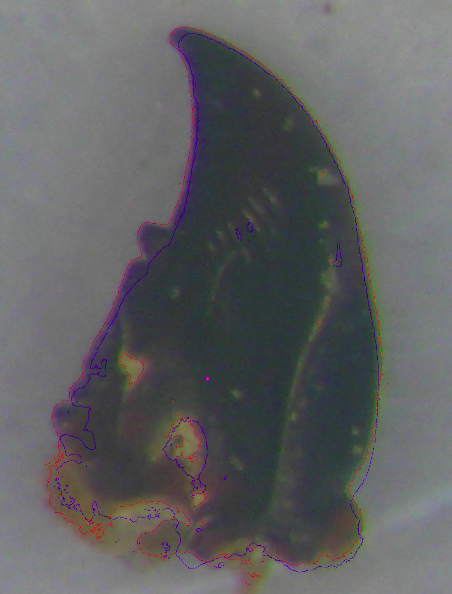
\includegraphics[width=0.3\textwidth]{./images/pca1}}~~
\subfloat[PCA with noises]{\label{figpca2}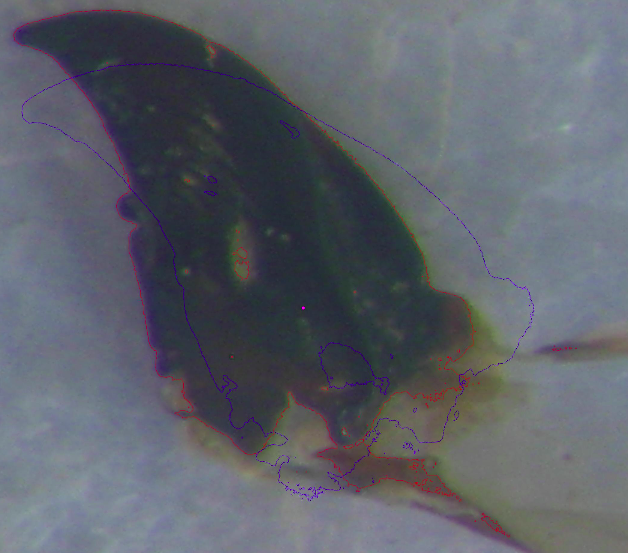
\includegraphics[width=0.4\textwidth]{./images/pca2}}
\caption{The result after applying the PCA}
\label{figpca}
\end{figure}
\subsection{PCA Iteration (PCAI)}
PCA method is a simplest method to align two images. However, PCA is more influenced by noises(see figure \ref{figpca}). Based on the idea of PCA method, PCAI try to apply the PCA on the interested data of the input.\\[0.2cm]
The solved problem in PCAI is the same with other difference registration methods. With two set of data input, specify curve points, we want to register two images with best matches. In PCAI method, firstly, PCA is applied on all two set of data for having the first sight of data. Secondly, the data is sorted followed one of coordinates of data points. The interested data is taken up with a half of data points which are sorted. Thirdly, an iteration will be executed to match the data. For each iteration, we re-compute the principal component of scene data and compare with the model. The iteration will be terminated when the difference position between two images is smallest (see figure \ref{figpcai}).\\[0.2cm]
\begin{figure}[h!]
\centering
\subfloat[Image alignment with PCA]{\label{figpcai1}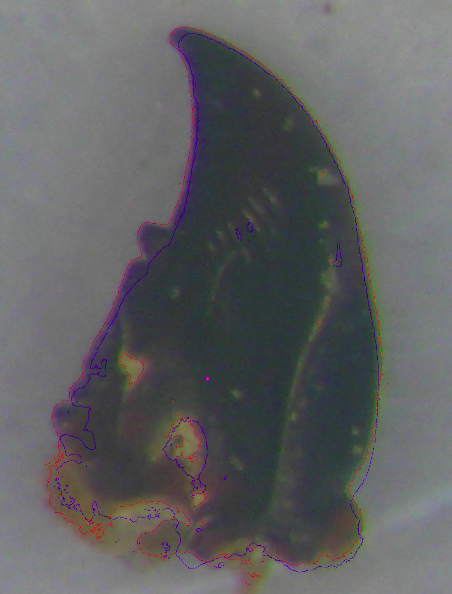
\includegraphics[width=0.4\textwidth]{./images/pca1}}~~
\subfloat[Image alignment with PCAI]{\label{figpcai2}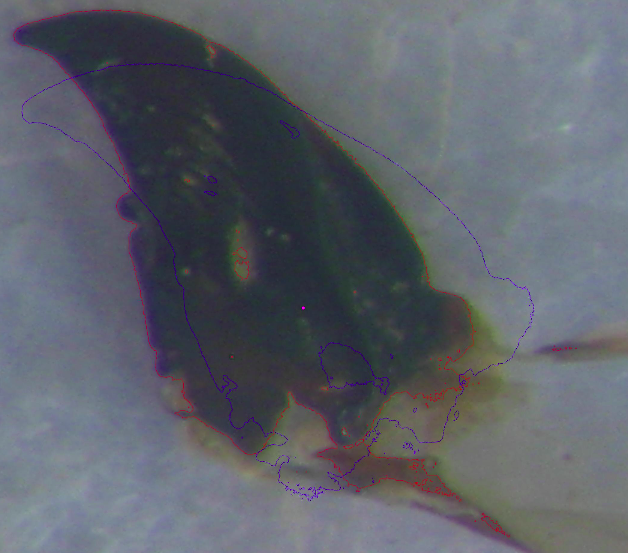
\includegraphics[width=0.4\textwidth]{./images/pca2}}
\caption{Comparing the result between PCA and PCAI}
\label{figpcai}
\end{figure}
Beside applying PCAI to make the images are matched. PCAI can combine with other technique to estimate the landmarks, such as template matching. At beginning, PCAI is applied to match the images. At the end, for each manual landmarks on the model, we apply the template matching to estimate the location of landmarks on scene image. 
\subsubsection{Result}
The combining between PCAI and template matching is experimented on two datasets of mandible (left and right mandible). For each set of data, it was divided into two sub-sets followed the size of objects. The model is chosen for each sub-set. The estimated landmarks coordinates are used to compute the centroid size of the mandibles. The results are compared with the centroid size of manual landmarks. In general, the success rate of the method is \textbf{90.56\%} for left mandible and \textbf{94.48\%} for right mandible (see figure...). On each sub-set of left mandible, the success rate of sub-set 1 is \textit{87.18\%} and \textit{97.80\%} for sub-set 2 (see figure). And \textit{94.52\%} and \textit{94.37\%} are success rates of sub-sets on right mandible(see figure).
Although the result from the method is good but it depends much on the result of segmentation. If the segmentation is not good and have many noises, the result of the method will be affected.
\subsection{Singular value decomposition (SVD)}
The PCA method is more effected by the noise, instead of using all the curve points, SVD just using a subset of points by optimal alignment between corresponding points of model and scene. Assume that \texttt{M} is a subset of the model points, \textbf{S} is a subset of the scene points and $p_i \in M, q_i \in S$ are two corresponding points. We would like to find the matrix transformed \textbf{R} so that the pair-wise distances between the corresesponding points is minimum. The pairwise distance is indicated by equation (\ref{eqpwdistance}).
\begin{center}
\begin{equation}\label{eqpwdistance}
	E = \sum_{i=1}^{n} {\|q_i - p_i^{'}\|}
\end{equation}
\end{center}
Where:
\begin{itemize}
	\item \textit{n}: is number of corresponding points
	\item \textit{$q_i$}: point of scene
	\item \textit{$p_i^{'}$}: point of model which corresponding with \texttt{$q_i$}
\end{itemize}
In detail, SVD method includes the following steps:
\begin{itemize}
	\item Calculate the cross covariance matrix: $M = P.Q^T$, where $P(Q)$ are matrix with i-th column is vector $p_i - c_T$ ($q_i - c_S$),
	\item Compute the singular value decomposition of matrix $M$: \textbf{$M = U.W.V^T$}. Where:
	\begin{itemize}
		\item U,V are \textit{m} x \textit{m} orthonormal matrices
		\item W is a diagonal \textit{m} x \textit{m} matrix with non-negative entries.
	\end{itemize}
	\item Indicate the orthonormal matrix (rotation matrix) $R = V.U^T$
\end{itemize}
\subsubsection{Result}
SVD method is solving the noise problem of PCA by using a set of corresponding points. The result obtained by applying the SVD also better PCA. But a disadvantage of SVD is requiring a accurate correspondences set of points which are usually not available.
\subsection{Iterative closest point (ICP)}
Based on the advantage and disadvantage of PCA and SVD. ICP combines two previous methods. The idea of ICP is using PCA to intial guess of correspondences and repeating SVD to improve correspondences. The steps of ICP are:
\begin{itemize}
	\item Transform the model by PCA aligment
	\item For each transformed model point, assign the closest scene point as its corresponding point. Align model and scene by SVD
	\item Repeat the step (2) until a termination criteria is met.
\end{itemize}
	\chapter{Software}
\section{The software architecture}
The architecture of program is followed 3-tier model. There-tier architecture is an architecture that each tier is designed, developed and maintained as independent. The advantage of this architecture is intended to allow any upgraded or replaced independent between the tiers. When user want to change the requirements or technology of a tier, it will non-affect to other tiers.\\[0.3cm]
The architecture of three-tiers includes:
\begin{itemize}
	\item \textbf{Data tier}: includes the classes which were designed for the data structure of program. It also provides the persistence mechanism to access the data.
	\item \textbf{Logic tier}: controls the functionality of application by performing detailed processing.
	\item \textbf{Presentation tier}: displays information related to user. It is a layer which received the require from user to program or return the result from program to user. 
\end{itemize}
\begin{figure}[h]
	\centering
	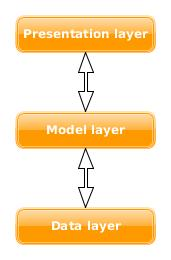
\includegraphics[scale=0.7]{images/software_3tiers}
	\caption{Three-tiers model}
	\label{fign3iters}
\end{figure}
\section{The modules}
The MAELab software mainly includes four modules: \textbf{segmentation}, \textbf{histograms}, \textbf{pht} and \textbf{correlation}. Besides, the software also includes the other modules to support for the main modules. The relation between the modules in the software is shown in figure \ref{fignsmodules}.
\begin{figure}[h]
	\centering
	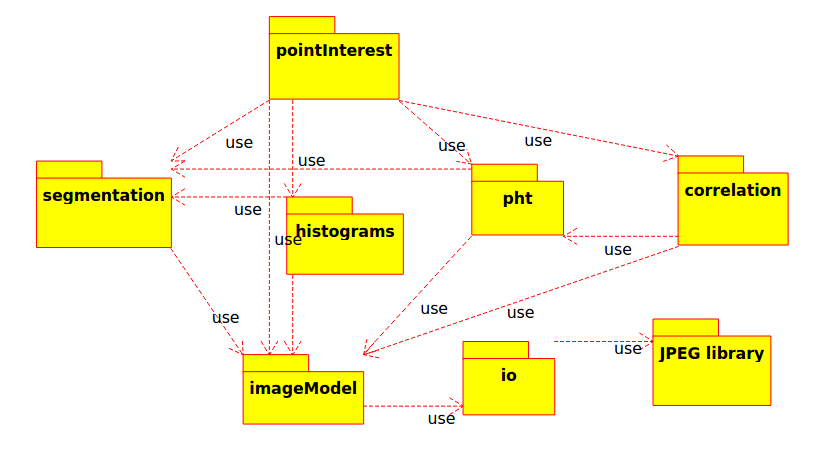
\includegraphics[scale=0.5]{images/modules}
	\caption{Three-tiers model}
	\label{fignsmodules}
\end{figure}
The functions of each modules is describing as followed:
\begin{itemize}
	\item \textbf{io} module: Implement the functions to read and write file. It includes the \textbf{JPEG library} that used to decode and encode the JPEG image.
	\item \textbf{imageModel} module: Represent the data structure of the image.
	\item \textbf{segmentation} module: Implement the segmentation methods on image.
	\item \textbf{histograms} module: Contains the methods to compute the geometric histogram of the image.
	\item \textbf{pht} module: Describe the probabilistic hough transform duration.
	\item \textbf{correlation} module: Includes the template matching methods.
	\item \textbf{pointInterest} module: Combine the result of the modules such as segementation, histograms,... to provide the adapter to other module or other software.
\end{itemize}
\section{The modules}
\section{The classes architecture}
\part{Deep learning}
	\chapter{Machine Learning}
Machine learning is a norm refer to teach the computer the abilities which are only done by the humans. A machine learning algorithm is an algorithm that is able to learn from data. Most of machine learning algorithms can be divided into two categories: supervised learning and unsupervised learning algorithms. \\
A machine learning algorithm is built based on the tasked for a machine learning system. We have many kinds of task can be solved with machine learning. Some of common machine learning tasks include the following:
\begin{itemize}
	\item \textit{Classification}: In this type of task, the computer is asked to indicate a category in k category which the input belongs to. To solve this task, the learning algorithm uses a function $y=f(x)$, the model assigns the input described by vector $x$ to a category identified by score y.
	\item \textit{Classification without input}: A challenge of classification is missing the input vectors. In this case, to solve the classification task, the learning algorithm only has to define a single function mapping from a vector input to a category output. When some of inputs are missing, instead of providing a single classification function, the learning algorithm must learn a set of functions. Each function corresponds to classifying x with different subset of its inputs missing.
	\item \textit{Regression}: the computer program is asked to predict a numerical value given some input.
	\item \textit{Transcription}: machine learning system is asked to observe a relatively unstructured representation of some kind of data and transcribe it into discrete, textual form.
	\item \textit{Translation}: The input already contains the sequence of symbols in some languages, the computer program must convert it into the sequence of symbols of other languages.
	\item \textit{Structure output}: involve any task where the output is a vector with important relationships between the different elements.
	\item \textit{Anomaly detection}
	\item \textit{Synthesis and sampling}: The program is asked to generate the new example that are similar with the training data.
	\item \textit{Imputation of missing value}: The algorithm mus provide a prediction of the values of the missing entries in a new example.
	\item \textit{Denoising}
	\item \textit{Density estimation or probability mass function estimation}
\end{itemize}
\section{Supervised learning algorithms}
\section{Unsupervised learning algorithms}
\section{Stochastic Gradient Descent}
	\chapter{Classification}
Classification is a most of important task in machine learning. In classification, a function is constructed to determine the category of the input. Generally, the model of classification as following:

The process of classification includes two steps:
\begin{enumerate}
	\item \textbf{Training}: Use the \textbf{training set} to learn what every object of a class looks like. This duration is called training a classifier or learning a model. The training set is a set with the objects which have labeled with specific category.
	\item \textbf{Evaluation}: To evaluate the quality of the classifier. We use a new set \textbf{(test set)} of the objects and try to ask the classifier predict the category of the object in the test set.
\end{enumerate}
In the content of this chapter, we will discuss about the classification techniques, especially, linear classification which technique has used more in neural network and deep learning.
\section{Nearest Neighbour Classifier}
The first approach to Classifier, we will develop Nearest Neighbour Classifier. This classifier do not have any relation with deep learning or convolutional networks, but it will help us to have an overview about classification problem.\\[0.2cm]
The idea of Nearest Neightbour Classifier is comparing each image in test data set with all image in training data set and predict the label of closet training image. And one of simplest methods to compare two images is comparing each pixels of two images and sum of all the differences. Assum that we have two vector \textbf{$I_1$}, \textbf{$I_2$} presented for two images, the equation to compare two images is following (called \textbf{L1 distance}):
\begin{equation}
	d_1(I_1,I,2)=\sum_{p}|{I_1}^p - {I_2}^p|
\end{equation}
Actually, we have many ways to compute the distances between two image. Instead of using L1 distance, we can use \textbf{L2 distance}, which has indicated by square root of euclidean distance between two vectors. The form of L2 distance as: 
\begin{equation}
	d_2(I_1,I,2) = \sqrt{\sum_{p}{({I_1}^p - {I_2}^p)}^2}
\end{equation}
For example, this is a way to compute distace between two images  (fig. \ref{fignncl1}):
\begin{figure}[h]
	\centering
	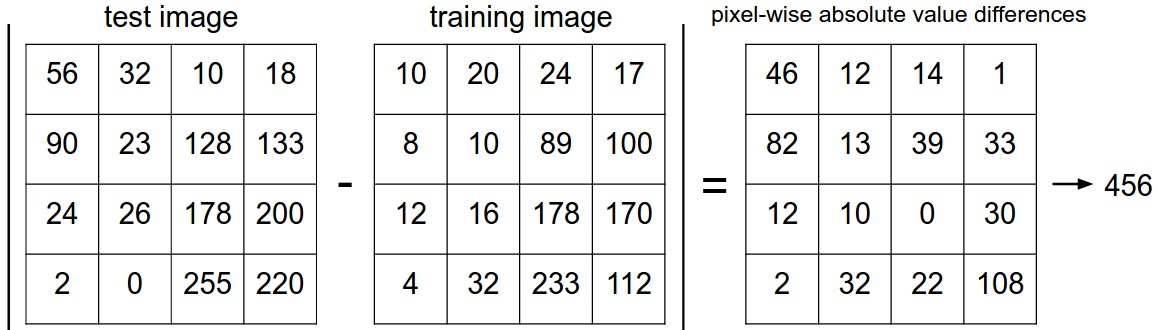
\includegraphics[scale=0.3]{images/nncl1.jpeg}
	\caption{An example used \textbf{L1 distance} to compare two images}
	\label{fignncl1}
\end{figure}
\section{K-Nearest Neighbour Classifier}
In the case of Nearest Neighbour Classifier, we just determine only one closest image in the training data with the test image when we wish to make a prediction. It means that we need some images in training data set that closest with the test image. In this case, we can use the \textbf{k-Nearest Neighbour Classifier}. The idea of this method is finding top \textbf{k} closest images instead of singel closest image (hence, when k = 1, we recover the Nearest Neighbour Classifier).\\[0.2cm]
In practice, what is the best value of k that we should to use? Besides that, we have many choices for  compute the distance between two images different with  L1 distance, L2 distance. The method called \textbf{hyperparameters} is vary for this work. This method comes in the design of many Machine Learning algorithsm, and it is used to choose the setting values. We should try out many different values and  see what works best. This is the idea, but we must be done vary carefully. Another noticed that, we do not try to evaluate on test data set with each \textit{k}. After having the \textit{k}, we evaluate on the test set only a single time, at the end of procedure.\\[0.2cm]
The idea is spitting the training data set in two subsets: the first subset is used to training, the other subset is used to validate (called \textbf{validation set}). The validation set is used as the test set to indicate the value of k. At the end of procedure, we could determine values of k work best. We would then use this value and evaluate once on the actual test set.\\[0.2cm]
In summary, split the training set into training set and validation set. use validation ton tune all hyperparameters. At the end run a single time on the test set and evaluate the result.
\section{Linear Classification}
The (k-)Nearest Neighbour Classifier had introduced about the problem of Image classification, which is predicting the label to an image from a fixed set of labels. But with the these methods, we must spend more time with large datasets an the cost for classifying is expensive. Another classification methods is known as \textbf{linear classification} which is the core of neural networks.
The linear classification has two main components: 
\begin{itemize}
	\item \textbf{Score function}:  which used to map the raw data to score of a category.
	\item \textbf{Loss function}: that quantifies the agreement between predict score and the truth category of the data.
\end{itemize}
The simplest function of a linear mapping is:
\begin{equation}
	y = f(x_i,W,b) = Wx_i + b
\end{equation}
Where:
\begin{itemize}
	\item $x_i$ is the raw data, \textit{example: an image}.
	\item $W$: a matrix parameter, called \textbf{weight} matrix
	\item $b$: vector, called \textbf{bias} vector
	\item $y$: score when consider the data $x_i$ belongs to a category.
\end{itemize}
In equation above, the input image \textbf{$x_i$} is fixed but we can control the setting of parameters \textbf{W and b}. Our goal is setting the parameters that the computing score match with the truth labels of image.
\begin{figure}[h]
	\centering
	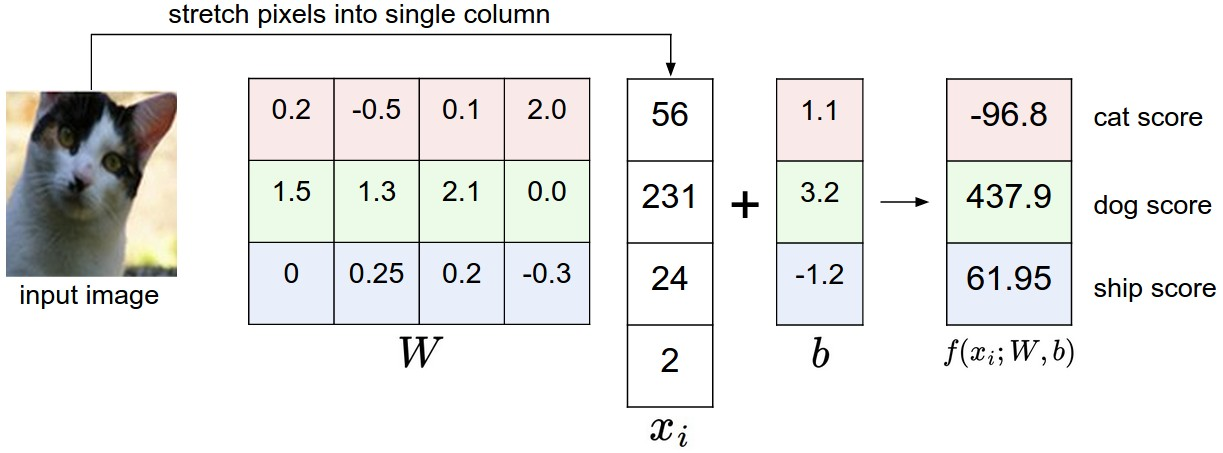
\includegraphics[scale=0.3]{images/lncex}
	\caption{An example of mapping an image to a class scores}
	\label{figlncex}
\end{figure}~\\
In training process, it is a little cumbersome to keep two sets of parameters (W,b) separately. A commonly trick is used to combine two sets of parameters into a single matrix that holds both of them by extending a vector \textbf{$x_i$} with one additional dimension and keep the constant defaut 1. Now, the new score function will be:
\begin{equation}
	y = f(x_i,W,b) = Wx_i
\end{equation}
Visualation of new score function:
\begin{figure}[h]
	\centering
	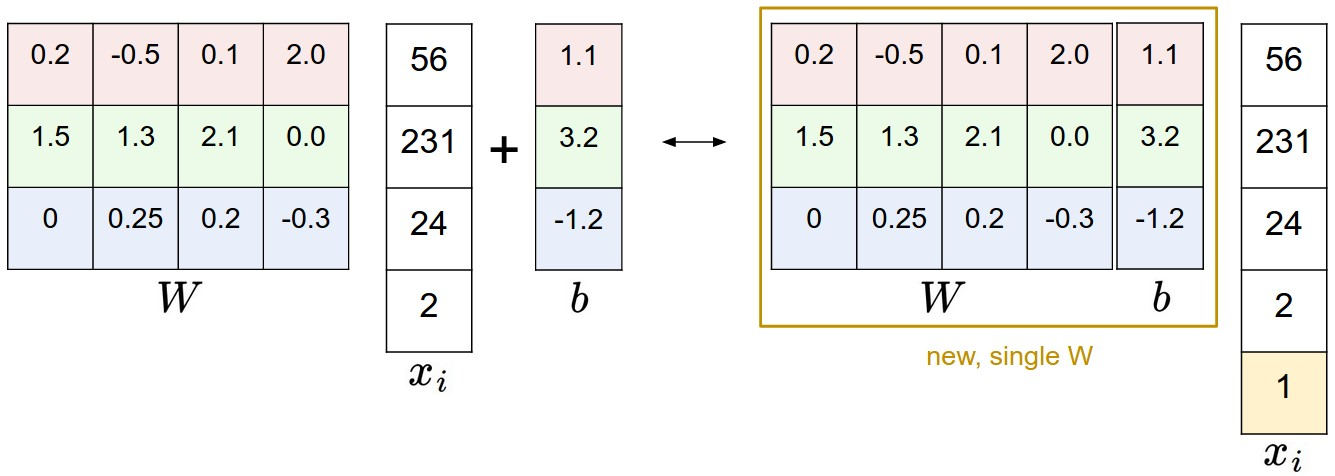
\includegraphics[scale=0.3]{images/lncba}
	\caption{An example of bias trick}
	\label{figlncex}
\end{figure}~\\
As described, we defined a score functions from a pixels value of an image to class scores with set of parameters \textbf{W}. Moreover, we need to control over parameters W such that the class scores are consistent with the ground truth labels in the training data. But not all cases are perfect, the class scores just near with the score of truth labels. So, we are going to measure the wrong with a \textbf{loss function}. Intuitively, the loss will be high if we are doing a poor classifier, ant it will be low if we are doing well. Multicalss Support Vector Machine (SVM) and Softmax function are two commonly methods for this purpose.
\subsection{Multiclass Support Vector Machine loss}
A commonly way to define the loss function called the \textbf{Multiclass Support Vector Machine} (SVM) loss. SVM loss is set up a margin $\Delta$ for the incorrect class scores. It means that SVM loss function wants the score of the correct class to be greater than the incorrect class (predict score) by at leat $\Delta$. If this is not the case, we will accumulate the loss.\\[0.2cm]
The SVM loss for the i-th is formalized as follows:
\begin{equation}
	L_i = \sum_{j \neq y_i }max(0,s_j - s_{y_i} + \Delta)
\end{equation}
Where:
\begin{itemize}
	\item $s_j$ is the score of $x_i$ for j-th class
	\item $s_{y_i}$ is the score of correct class
	\item $\Delta$ is margin 
	\item $max(0,-)$ is thresholding to zero, called hinge loss.
\end{itemize}
For example, we have three predict scores of an image $x_i$ like \textbf{$s = [14,-9,11]$}, and the first class is true class of $x_i$. Assume that $\Delta$ is 10. The SVM loss of this case is following:
\begin{center}
$
	L_i = max(0,-9 - 14 + 10) + max (0,11 - 14 + 10) = 0 + 7 = 7
$
\end{center}
\subsection{Softmax classifer}
The other popular choice to define the loss function  is the \textbf{Softmax classifier}. Unlike SVM which treats the output of score function for each class, the Softmax classifier give a sightly more intuitive output and use the probabilistic description. Instead using theshold zero function as SVM, Softmax is using a \textbf{cross-entropy loss} for \textit{hingle loss}, which has the form.
\begin{equation}
	L_i = -log(\frac{e^{f_{y_i}}}{\sum_j{e^{f_j}}})
	\label{softmax}
\end{equation}
Where: $f_j$ is the j-th element of vector of class scores \textbf{$f$}.\\[0.2cm]
In formula \ref{softmax}, the function $f_j(z) = \frac{e^{z_j}}{\sum_k{e^{z_k}}}$ is called the softmax function. This formula turns the predict scores into probabilistic values (Noticed that sum of all \textbf{$f_j(z) $} is 1).\\[0.2cm]
The cross-entropy between a correct distribution \textbf{p} and an estimated distribution \textbf{q} is defined as:
\begin{equation}
	H(p,q) = -\sum_x{p(x)log(q(x))}
\end{equation}
The Softmax classifier is minimizing the cross-entropy between the estimated socre and true score. At the end, the loss of training process is the average of cross-entropy.
\begin{equation}
	L = \frac{1}{N}\sum_i(H(p,q))
\end{equation}
The image \ref{figsvmsf} describes an example for a comparison between SVM and Softmax:
\begin{figure}[h]
	\centering
	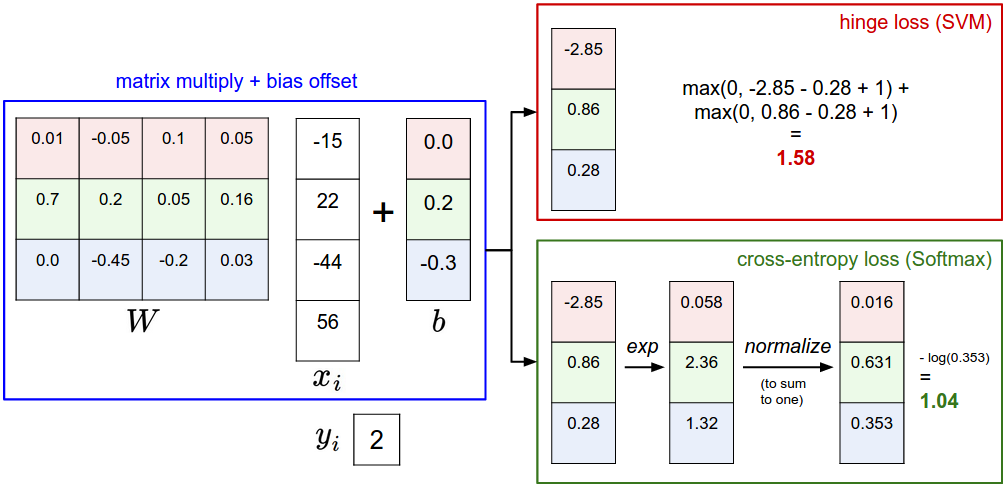
\includegraphics[scale=0.45]{images/svmsf}
	\caption{An example about SVM and Softmax classifiers}
	\label{figsvmsf}
\end{figure}~\\[2.5cm]
Both SVM and Softwax compute the same score of vector f. The difference is the way to present the score f: SVM uses the margin and Softmax uses probabilistic. In practice, the SVM and Softmax are usually used and compared in the machine learning systems.
\section{How to determine the value of W and b?}
\section{Backpropagation}
	\chapter{Deep Network}
\section{Neural network}
\subsection{Neural}
The basic components of the brain is a neuron. For the ordinary man, we have billion neurons in the human nervous system, and they are connected by the billion of synapses. Each neuron receives input signals from its dendrites and procedures output signals along its axon.\\[0.2cm]
In the computational model of a neuron, the signals travel along the axons interact multiplicatively with the dendrites of the other neuron based on the synaptic strength at the synapse. The synaptic strength are learnable and control the strength at influence or inhibitory of one neuron on another. In basic mode, the input signals are summed and compared with a threshold value. If the sum is greater than threshold value, the neuron can fire, sending a spike along its axon. Actually, we have many firing rate (called activation function) at a neuron, and the common choice of activation function is the \textbf{sigmoid funciont $\sigma$}, because it take a real-valued input and squashes it to range between 0 and 1. The image () show the model of a neuron:
\begin{figure}[h]
	\centering
	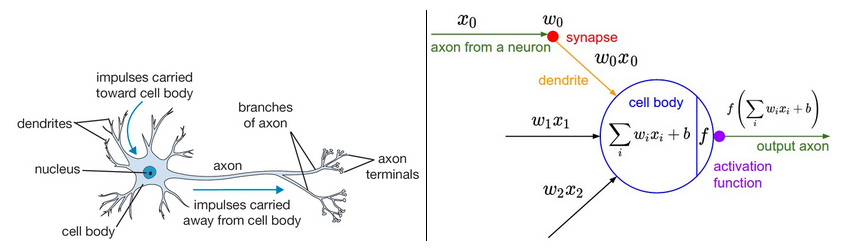
\includegraphics[scale=0.5]{images/neurons.png}
	\caption{A drawing of a biological neuron and its mathematical model}
	\label{fignneuron}
\end{figure}
Some activation functions which we can use:
\begin{itemize}
	\item \textbf{Sigmoid function}:
		\begin{equation}
			\sigma(x) = \frac{1}{1+e^{-x}}
		\end{equation}
	\item \textbf{Tanh}
		\begin{equation}
			tanh(x) = 2\sigma(2x) - 1
		\end{equation}
	\item \textbf{ReLU}
		\begin{equation}
			f(x) = max(0,x)
		\end{equation}
	\item \textbf{Maxout}:
		\begin{equation}
			f(w^Tx + b) = max({w_1}^Tx + b_1,{w_2}^Tx + b_2)
		\end{equation}
\end{itemize}
\section{The architecture of neural networks}
\begin{figure}[h]
	\centering
	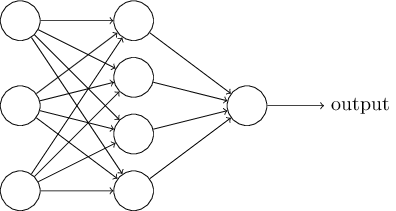
\includegraphics[scale=0.5]{images/neuron}
	\caption{A model of neural networks}
	\label{fignnnetworks}
\end{figure}
The image \ref{fignnnetworks} show a simple model of neural networks. The leftmost layer in this network is called the input layer, the rightmost layer is called the output layer. The neurons within the input layer are called input neurons, the neurons from output layer are called output neurons. The middle layer is called a hidden layer. The network in example \ref{fignnnetworks} has just a single hidden layer, but many networks have multiple hidden layers. When design the network, the input and the output are often straightforward. It means that the neural networks is designed where the output form one layer is used as the input to the next layer, there are no loops in the network, it always feed forward, never feed back (called feedforward networks).\\[0.2cm]
So, the neural network includes many layers are designed as an directred acyclic graph from the intput to the output layer. The output of previous layer is used as the input of the next layer. At each layer excepts the output layer, the output is indicated by a activation function (i.e loss, tanh,...). The size of a neural network can be to compute as the number of neurons, or the number of parameters.
\section{Deep network}
	\chapter{Convolutional Neural Network}
Convolutional Neural Networks (CNNs) are similar with the original of Neural Networks. Neural Networks receive an input and pass it through a series of hidden layer. Each hidden layer is made from a set of neurons, where each neuron is full connected with all neurons of previous layer. Actually, the neural networks do not scale well to full images...
\section{Architecture}
A CNN is made from the layers. The common layers in CNN are convolutional, nonlinear, pooling and full connected layers. CNN takes image as an input, pass it through the series of layers and get an ouput. Each layer has a difference function to transform the input to another layer. 
\subsection{Convolutional layer}
\subsection{Pooling layer}
\subsection{Full connected layer}
\section{Testing}
\part{Conclusion}
	\chapter{Discussion}
	\chapter{Conclusion}
\bibliographystyle{unsrt}
\bibliography{includes/references}
\end{document}